\documentclass{standalone}
\usepackage{tikz}
\usepackage{ctex}
\setCJKmainfont{Noto Serif CJK SC}
\usepackage{mhchem,siunitx}
\usetikzlibrary{patterns}
\begin{document}
\small
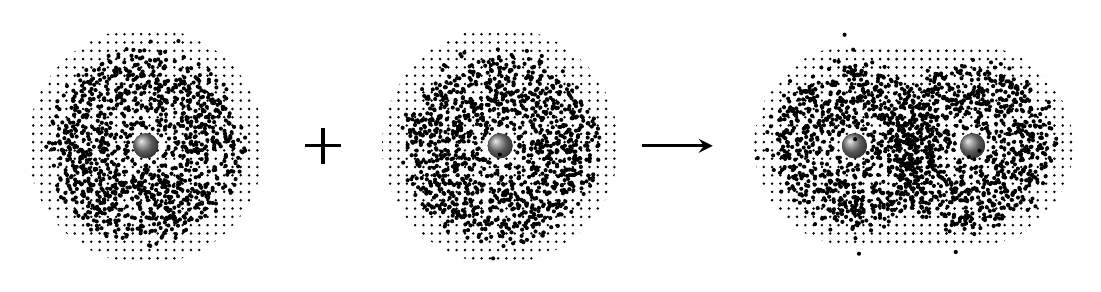
\begin{tikzpicture}[>=stealth,scale=1.5]
  \begin{scope}
    \fill[pattern = dots](0,0)circle(1);
    \fill[ball color=gray] (0,0)circle(3pt);
    \foreach \x in {1,2,...,30} 
      {
        \fill(360*rnd:rnd)circle(0.5pt);
        \foreach \y in {0.2,0.3,...,0.9,0.8,0.7,0.7,0.7,0.6,0.6,0.65,0.55,0.5,0.45,0.4,0.35}
        {
          \fill(360*rnd:\y+0.05*rnd)circle(0.5pt);
          \fill(360*rnd:\y-0.05*rnd)circle(0.5pt);
        }
      }
  \end{scope}
  \begin{scope}[xshift=3cm]
    \fill[pattern = dots](0,0)circle(1);
    \fill[ball color=gray] (0,0)circle(3pt);
    \foreach \x in {1,2,...,30} 
      {
        \fill(360*rnd:rnd)circle(0.5pt);
        \foreach \y in {0.2,0.3,...,0.9,0.8,0.7,0.7,0.7,0.6,0.6,0.65,0.55,0.5,0.45,0.4,0.35}
        {
          \fill(360*rnd:\y+0.05*rnd)circle(0.5pt);
          \fill(360*rnd:\y-0.05*rnd)circle(0.5pt);
        }
      }
  \end{scope}
  \begin{scope}[xshift=6cm]
    \fill[pattern = dots](0.85,0.85)--(0,0.85)arc(90:270:0.85)--(0.85,-0.85)--cycle;
    \fill[ball color=gray] (0,0)circle(3pt);
    \foreach \x in {1,2,...,30} 
      {
        \fill(360*rnd:rnd)circle(0.5pt);
        \foreach \y in {0.2,0.3,...,0.7,0.7,0.6,0.6,0.65,0.55,0.5,0.45,0.4,0.35}
        {
          \fill(360*rnd:\y+0.05*rnd)circle(0.5pt);
          \fill(360*rnd:\y-0.05*rnd)circle(0.5pt);
        }
      }
  \end{scope}
  \begin{scope}[xshift=7cm]
    \fill[pattern = dots](0,0.85)--(-0.85,0.85)--(-0.85,-0.85)--(0,-0.85)arc(-90:90:0.85)--cycle;
    \fill[ball color=gray] (0,0)circle(3pt);
    \foreach \x in {1,2,...,30} 
      {
        \fill(360*rnd:rnd)circle(0.5pt);
        \foreach \y in {0.2,0.3,...,0.7,0.7,0.6,0.6,0.65,0.55,0.5,0.45,0.4,0.35}
        {
          \fill(360*rnd:\y+0.05*rnd)circle(0.5pt);
          \fill(360*rnd:\y-0.05*rnd)circle(0.5pt);
        }
      }
  \end{scope}
  \draw[very thick](1.35,0)--(1.65,0)(1.5,-0.15)--(1.5,0.15);
  \draw[very thick,->](4.2,0)--(4.8,0);
\end{tikzpicture}
\end{document}